\documentclass{article}
\usepackage{graphicx} % Required for inserting images
% \setlength{\parindent}{0cm} 
\usepackage{caption}
\usepackage{subcaption}
\usepackage[%  
    colorlinks=true,
    pdfborder={0 0 0},
    linkcolor=red
]{hyperref}
\usepackage{geometry}
 \geometry{
 a4paper,
 total={170mm,257mm},
 left=20mm,
 top=20mm,
 }
\usepackage{hyperref}
\usepackage{blindtext}
\usepackage{titlesec}

\usepackage{biblatex}
\addbibresource{references.bib}


\usepackage{tcolorbox}
\tcbuselibrary{minted,breakable,xparse,skins}

\definecolor{bg}{gray}{0.95}
\DeclareTCBListing{mintedbox}{O{}m!O{}}{%
  breakable=true,
  listing engine=minted,
  listing only,
  minted language=#2,
  minted style=default,
  minted options={%
    linenos,
    gobble=0,
    breaklines=true,
    breakafter=,,
    fontsize=\small,
    numbersep=8pt,
    #1},
  boxsep=0pt,
  left skip=0pt,
  right skip=0pt,
  left=25pt,
  right=0pt,
  top=3pt,
  bottom=3pt,
  arc=5pt,
  leftrule=0pt,
  rightrule=0pt,
  bottomrule=2pt,
  toprule=2pt,
  colback=bg,
  colframe=orange!70,
  enhanced,
  overlay={%
    \begin{tcbclipinterior}
    \fill[orange!20!white] (frame.south west) rectangle ([xshift=20pt]frame.north west);
    \end{tcbclipinterior}},
  #3}
\usepackage{amsmath}

\title{First model of spacetime around binary black holes}
\author{Jordan Moncrieff}
\date{June 2023}

\begin{document}

\maketitle

\tableofcontents

% \begin{abstract}
%     In this document, I summarise some of the work I have done at the start of the winter internship. 
%     This involves looking at the simplest scenario of binary black hole (BBH) mergers - involving gravitational wave emissions and frame dragging effects to first order - i.e. the basic ingredients that I suspect are required for reconnection to occur. 
    
%     In section \ref{sec:Model} I explain the basic setup of my model, and derive the equations of motion for the simple system. Then in section \ref{sec:Numerics} I simulate this system numerically in Python, exploring the behavior of the system - some of the code I wrote can be found in the appendix section \ref{sec:Python code}. This is followed by section \ref{sec:Analytic}, where I employ approximation methods to try to analytically analyse the system, proving some of the behavior I observed in the preceding section (I have not actually done this yet, but I plan to). Finally, in section \ref{sec:Limitations and next steps} I describe the limitations of my model, as well as the next steps required to make improvements.
    
%     This work extends what was done in \cite{2010ApJ...724...39S}, where they only considered GW emission. This document is a work in progress, there are parts that are unfinished and or contain errors.

\begin{abstract}
    

In this document, I provide a summary of the work I have undertaken during the initial stages of the winter internship. This document outlines a basic model for binary black hole (BBH) mergers, specifically exploring gravitational wave emissions and frame dragging effects to a first-order approximation. I suspect these are the necessary ingredients required for gravitational reconnection to occur.

The document is structured as follows:
\begin{itemize}
\item In Section \ref{sec:Model}, I outline the basic setup of my model and derive the equations of motion for the simplified BBH system.
\item Section \ref{sec:Numerics} describes the numerical simulations conducted using Python, allowing for an exploration of the system's behavior. The appendix (section \ref{sec:Python code}) contains some of the relevant code that I have written.
\item In Section \ref{sec:Analytic}, I discuss the application of approximation methods to analytically analyze the system, providing insight into the observed behavior. I have done this section yet, but I plan to.
\item Finally, Section \ref{sec:Limitations and next steps} addresses the limitations of my model and proposes the subsequent steps necessary for further enhancements.
\end{itemize}

This work builds upon the previous research conducted in the paper \cite{2010ApJ...724...39S}, which solely focused on gravitational wave emission. This document is a work in progress, certain sections remain incomplete and contain errors.
\end{abstract}



\section{Basic model}\label{sec:Model}

\subsection{Essential ingredients}

We follow the tried an true theoretical physics and applied mathematics approach of simplifying the problem as much as possible, while still maintaining the essential features of the problem. We eventually want a full general relativistic model of a binary black hole merger, and we want to see if this leads to a reconnection of gravitational field lines. The problem is, general relativity is hard, not just for me, but for everyone. There is no analytic expression for the metric describing the gravitational field around or within binary black holes. This has lead Physicists to come up with different approximation schemes, as well as numerical relativity simulations. This is the long term goal of this project, but there is no reason to start at the end point, we first want a general idea of the problem before we start attacking it head on. This is the idea of this document.

As I have mentioned before, the defining property of BHs required for reconnection to occur is frame dragging. We also require a dynamical situation, but in classical Newtonian theory energy is conserved for binaries and so there is no evolution, thus we also require gravitational wave emission. So the most basic model must include these two effects, at least to first order.

\subsection{The model}

We start with two masses orbiting one another in a Keplerian orbit mutually attracting each other with a Newtonian potential. This is the classical two body problem, whose solution is well known. We can simplify the problem by considering the (non-inertial) reference frame rotating about the center of mass with angular frequency matching the orbital frequency of the binaries - this means the two masses are stationary in this reference frame. However, this non-inertial reference frame introduce three fictitious or pseudo-forces, namely centrifugal, Coriolis, and Euler forces. We then make this situation more similar to that of BBHs by introducing a variable angular frequency parameter, which decays according to what would be expected through energy losses via gravitational wave emissions. Finally, we add in an additional force from frame dragging, which to first order is given by the gravitomagnetic force.

It is well known from Classical mechanics (TODO: Derive this) that inside a reference frame (with coordinates $\vec{r}^{\prime}$) rotating with angular frequency $\vec{\omega}$ (with respect to the inertial coordinate frame, with coordinates $\vec{r}$) Newton's second law becomes

\begin{equation}
%Fix the weird looking prime
        \label{eq:Fictitious forces}
        m \ddot{\vec{r}}^{\prime} = \vec{F} - 2 m \vec{\omega} \times \vec{v}^{\prime} - m \dot{\vec{\omega}} \times \vec{r}^{\prime} - m \vec{\omega} \times \left(  \vec{\omega} \times \vec{r}^{\prime}  \right)
\end{equation}

Where $\vec{F}$ is the net external force, the first term $- 2 m \vec{\omega} \times \vec{v}^{\prime}$ is the \textit{Coriolis force}, the next term $- m \dot{\vec{\omega}} \times \vec{r}^{\prime}$ is the \textit{Euler force} associated with the changing rate of rotation, and the final term $- m \vec{\omega} \times \left(  \vec{\omega} \times \vec{r}^{\prime}  \right)$ is the \textit{centrifugal force}.

\begin{figure}
    \centering
    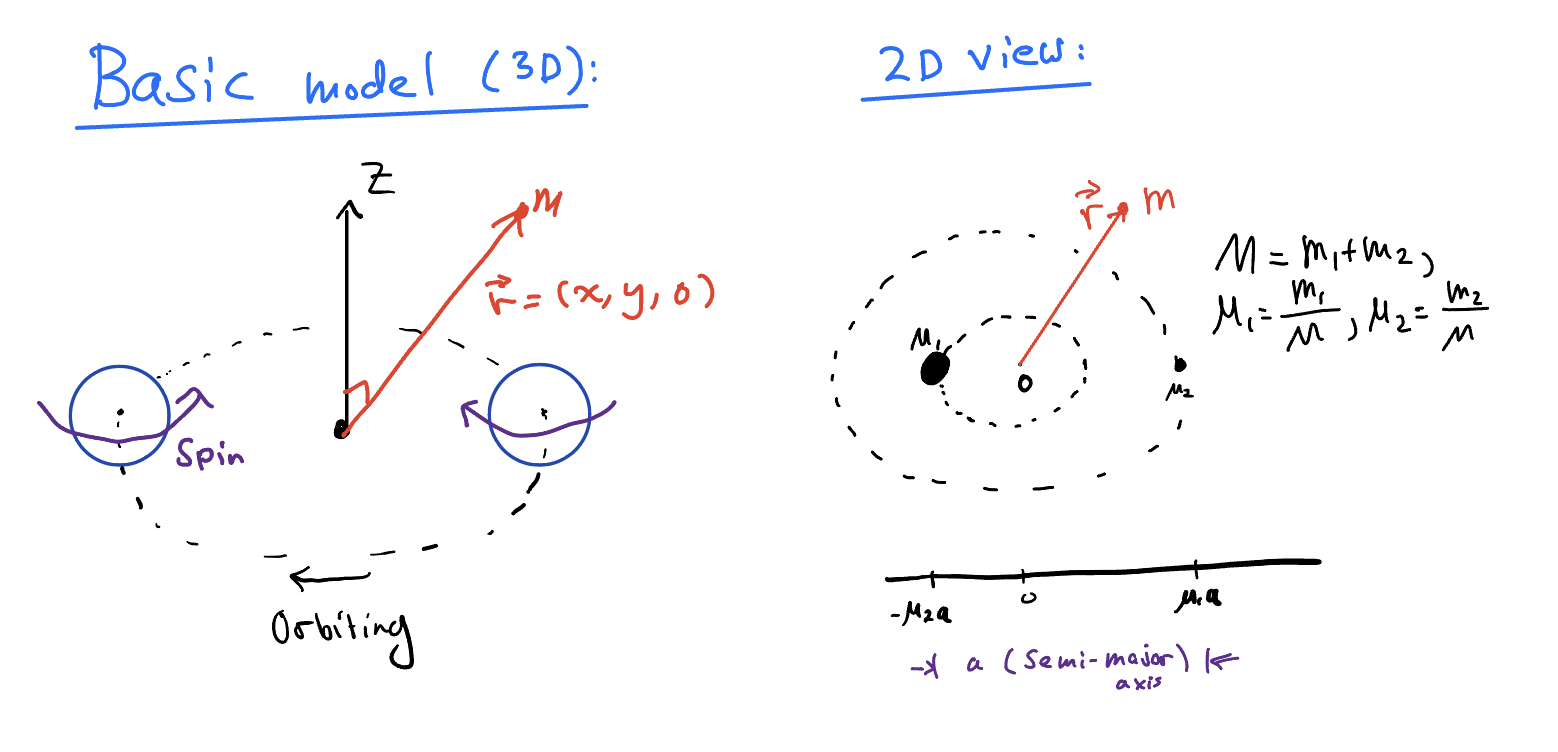
\includegraphics[width=0.75\textwidth]{images/basic_model_img.jpeg}
    \caption{The setup of basic model ...}
    \label{fig:basic model}
\end{figure}

Consider two point masses, $M_1$ and $M_2$ with $M_1 > M_2$ orbiting the common center of mass at the origin $(x,y)=(0,0)$, as depicted in figure \ref{fig:basic model}. Given the total mass $M_1+M_2=M$, we define the dimensionless masses $\mu_1=\frac{M_1}{M}$ and $\mu_2=\frac{M_2}{M}$, then in the rotating frame, the position of mass $M_1$ and $M_2$ is $(x_1, y_1)=(-\mu_2 a, 0)$ and $(x_2, y_2)=(+\mu_1 a, 0)$ respectively (it is easy to check that this ensures the centre of mass is at the origin). Kepler's third law states that the period of orbit $T$ of these masses is 

\begin{equation}
    T^2 = \frac{4 \pi^2}{G M} a^3
\end{equation}

Where $a$ is the semi-major axis of the resulting elliptical orbit. Since we are using units $G M=c=1$, we can write this equation as

\begin{equation}
    \label{eq:kepler's law}
    \omega = a^{-\frac{3}{2}}
\end{equation}

Where $\omega=\frac{2 \pi}{T}$ is the angular frequency of the orbits. Next, we consider adding a test particle into the resulting field (i.e. a mass small enough that it has no effect on the orbit of the larger masses) at the position $(x,y)$. In our reference frame rotating at angular frequency $\omega$, have the following forces acting on the test particle

\begin{enumerate}
    \item The pseudo-forces introduced by the angular frequency vector $\vec{\omega}=\omega \hat{z}$ (the direction of vector is given by the right hand rule, and the rotation is in the x-y plane).
    \item The gravitational force due to both masses (which add linearly in Newtonian mechanics). This is our \textit{gravito-electric} force.
    \item The force due to frame dragging, which we approximate as the linear superposition of two \textit{gravito-magnetic} forces coming from each masses.
\end{enumerate}

With some vector algebra, we can use equation (\ref{eq:Fictitious forces}) and apply them in Cartesian coordinates with $\vec{r}=(x,y,z)$ and $\vec{\omega}=(0, 0, \omega)$ to give the Coriolis, Euler, and Centrifugal forces:


\begin{align}
    \vec{F}_{\text{Coriolis}} &= -2 m \vec{\omega} \times \vec{v}^{\prime} \notag \\
    &= -2 m (0, 0, \omega) \times (\dot{x}, \dot{y}, 0) \notag \\
    &= (2 \omega \dot{y}, -2 \omega \dot{x}, 0) \notag \\
    \notag\\
    \vec{F}_{\text{Euler}} &= -m \dot{\vec{\omega}} \times \vec{r}^{\prime} \notag \\
    &= -m (0, 0, \dot{\omega}) \times (x, y, 0) \notag \\
    &= (-\dot{\omega} y, \dot{\omega} x, 0) \notag \\
    \notag\\
    \vec{F}_{\text{Centrifugal}} &= -m \vec{\omega} \times (\vec{\omega} \times \vec{r}^{\prime}) \notag \\
    &= -m (\vec{0} - \vec{r} (\vec{\omega} \cdot \vec{\omega})) \notag \\
    &= \omega^2 \vec{r} = \omega^2 (x, y, 0) \notag
\end{align}

Where we have restricted ourselves to the case where $z = \dot{z} = 0$, and in calculating the Centrifugal force we made use of the "BAC-CAB" vector identity.

\begin{equation}
    \vec{a} \times ( \vec{b} \times \vec{c}) = \vec{b} (\vec{a} \cdot \vec{c}) - \vec{c} (\vec{a} \cdot \vec{b})
\end{equation}

The force due to gravity is simply the sum of the Newtonian gravitational forces from each of the masses, given by 

\begin{equation}
    \vec{F}_\mathrm{gravity} = m \frac{-G m_1}{r_1^3} \vec{r_1} + m \frac{-G m_2}{r_2^3} \vec{r_2}
\end{equation}

Where the position vector of mass $m$ with respect to the positions of mass $m_1$ at $(-\mu_2 a, 0)$ and $m_2$ at $(\mu_1 a, 0)$ is $\vec{r_1} = (x+\mu_2 a, y, 0)$ and 
$\vec{r_2}=(x-\mu_1 a, y, 0)$ respectively. Since we have set $G M=1$, we can therefore find the acceleration $a_\mathrm{g}$ of the test particle due to gravity

\begin{equation}
    a_\mathrm{g} = (\mu_1 \frac{x+a \mu_2}{r_1^3} + \mu_2 \frac{x-a \mu_1}{r_2^3}, 
    \frac{\mu_1 y}{r_1^3} + \frac{\mu_2 y}{r_2^3}, 0)
\end{equation}

Finally, we add in the force on the test particle due to the gravito-electric field\footnote{I realised after doing this calculation that I did not account for the spin interaction between the primary and secondary masses, which is likeley important. I can not think of a straight foward fix to this.}. In the weak field of general relativity, the gravito-magnetic field at the location $\vec{r}$ due to a rotating mass of angular momentum $\vec{L}$ is (as shown in \cite{Moore}) given by 

\begin{equation}
    \label{eq: Gravitomagnetic field}
    \vec{B_g} = \frac{G}{2 c^2} \left[ \frac{\vec{L} - 3 \left(\vec{L} \cdot \vec{r} / r\right) \vec{r} / r}{r^3} \right]
\end{equation}

Resulting a mass current, generated by a mass $m$ moving with velocity $\dot{\vec{r}}$, experiencing a frame dragging force

\begin{equation}
    \label{eq: Force due to frame dragging in gravitomagnetism}
    \vec{F}_B = 4 m \times \dot{\vec{r}} \times \vec{B}_g
\end{equation}

We align the spins of the two masses in opposite directions within the z-axis, giving angular momenta $\vec{L}_1= L_1 \hat{z}$ and $\vec{L}_2= -L_2 \hat{z}$, this leads the term involving $\vec{L} \cdot \vec{r}$ vanishing (the motion is confined to the x-y plane). We can now 
calculate $\vec{F}_B$, using the cross products of the unit vectors $\hat{x} \times \hat{z} = -\hat{y}$ and $\hat{y} \times \hat{z} = \hat{x}$, we find the acceleration $\vec{a}_\mathrm{fd}$ on the test particle due to frame dragging

\begin{equation}
    \label{eq: Acceleration due to frame dragging}
    \vec{a}_\mathrm{fd} = \left(\frac{2 L_2}{r_2^3} \dot{y} \right) \hat{x} + \left( \frac{2 L_2}{r_1^3} \dot{x} \right) \hat{y}
\end{equation}

We also need to account for the fact that emission of gravitational waves results in the two masses falling towards one another as energy is lost from the system. This results in the angular frequency  (and by Kepler's law, the angular separation) decreasing, at a rate  (as shown in \cite{peters1964gravitational}) given by 

\begin{equation}
    \dot{\omega} = \frac{96}{5} \mu_1 \mu_2 \omega^{\frac{11}{3}}
\end{equation}

Adding all of these forces together, Newton's second law gives us the following system of coupled, non-linear, second order, ordinary differential equations


% \begin{align}
%     \ddot{x} &= 2 \omega \dot{y} + \omega^2 x + \dot{\omega} y - \left[   \mu_1 \frac{x+a \mu_2}{r_1^3} + \mu_2 \frac{x-a \mu_1}{r_2^3}  \right]  +\frac{2 L_2}{r_2^3} \dot{y}  \\

%     \ddot{y} &= -2 \omega \dot{x} + \omega^2 y - \dot{\omega} x - \left[ \frac{\mu_1 y}{r_1^3} + \frac{\mu_2 y}{r_2^3} \right]  + \frac{2 L_1}{r_1^3} \dot{x} \\

%     % \ddot{z} &= -\left[   \frac{\mu_1 z}{r_1^3} + \frac{\mu_2 z}{r_2^3}   \right]    \\

%     \dot{\omega} &= \frac{96}{5} \mu_1 \mu_2 \omega^{\frac{11}{3}}
    
% \end{align}

\begin{align}
    \ddot{x} &= 2 \omega \dot{y} + \omega^2 x + \dot{\omega} y - \left[ \mu_1 \frac{x+a \mu_2}{r_1^3} + \mu_2 \frac{x-a \mu_1}{r_2^3} \right] + \frac{2 L_2}{r_2^3} \dot{y} \label{eq:x dot dot} \\
    \ddot{y} &= -2 \omega \dot{x} + \omega^2 y - \dot{\omega} x - \left[ \mu_1 \frac{y}{r_1^3} + \mu_2 \frac{y}{r_2^3} \right] + \frac{2 L_1}{r_1^3} \dot{x} \label{eq:y dot dot}\\
    % \ddot{z} &= -\left[ \frac{\mu_1 z}{r_1^3} + \frac{\mu_2 z}{r_2^3} \right] \\
    \dot{\omega} &= \frac{96}{5} \mu_1 \mu_2 \omega^{11/3}
\end{align}

I would be extremely surprised if there was an analytic solution to this, so we need to either make approximations or simulate this numerically. I will do both of these, first by  numerically simulating this system in Python, and then by linearizing this equations around the fixed point at one of the  Newtonian Lagrange points.



%%%%%%%%%%%%%%%%%%%%%%%%%%%%%%%%%%%%%%%%%
%%%%%%%%%%%% Numerics %%%%%%%%%%%%%%%%%%%
%%%%%%%%%%%%%%%%%%%%%%%%%%%%%%%%%%%%%%%%%



\section{Numerical simulation of model}\label{sec:Numerics}

I have provided the Python code that I wrote to simulate the system in the appendix section (\ref{sec:Python code}). First, I will review some basics of Lagrange points in the Newtonian case.

%%%%%%%%%%%%%%%%%%%%%%%%%%%%%%%%%%%%%%%%%%%%%%%
%%%%%%%%%%%% Newtonian case %%%%%%%%%%%%%%%%%%%
%%%%%%%%%%%%%%%%%%%%%%%%%%%%%%%%%%%%%%%%%%%%%%%


\subsection{Lagrange points}

\subsubsection{Lagrange point stability}

\begin{figure}
    \centering
    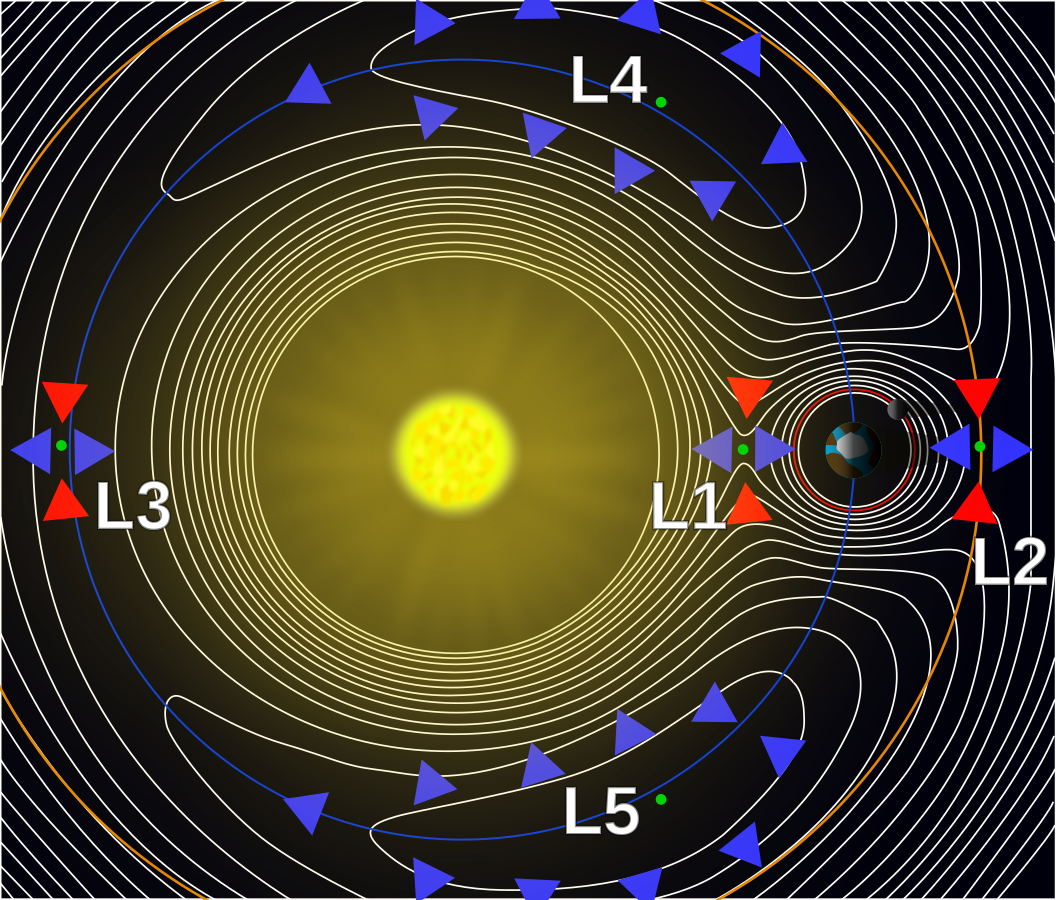
\includegraphics[width=0.8\textwidth]{images/1056px-Lagrange_points2.svg.png}
    \caption{Illustration of Largange points.}
    \label{fig:Lagraange points}
\end{figure}

The Lagrange points in a binary system refer to the five specific points in the orbital plane of the two-body system where a small object can maintain a stable or unstable position relative to the two larger bodies. The positions of these points is shown in figure \ref{fig:Lagraange points}.

Now, regarding stability: L1, L2, and L3 are unstable in the sense that a small perturbation will move the object away from the Lagrange point, and the object will not return. However, they are stable in a different sense: an object close to these points will stay close (though not in a fixed position) if it has a small "velocity" relative to the point. This is known as \emph{metastability}.

L4 and L5, on the other hand, are stable under small perturbations, provided the mass ratio of the two main bodies is greater than approximately 24.96. This condition is met for many significant cases, such as the Earth-Moon system and the Sun-Jupiter system. If an object is slightly perturbed from L4 or L5, it will move around the Lagrange point but not away from it.

The L1 point is metastable. This means that while an object at L1 might move away if perturbed, an object close to L1 will stay close if it is moving at a small relative speed. This is the principle behind the solar observatories SOHO and ACE, for example, which are in orbits designed to keep them close to the Sun-Earth L1 point.

\subsubsection{Astrophysical consequences}

Astrophysically, this property of metastability has interesting implications for angular momentum accretion. In the vicinity of the L1 point, matter can transition from one body to another due to gravitational forces. This is particularly important in binary star systems, where one star can accrete matter from its companion star if the companion overflows its Roche lobe - the region of space around a star where material is gravitationally bound to that star. The point at which this overflow occurs is often near the L1 point.

\begin{figure}
    \centering
    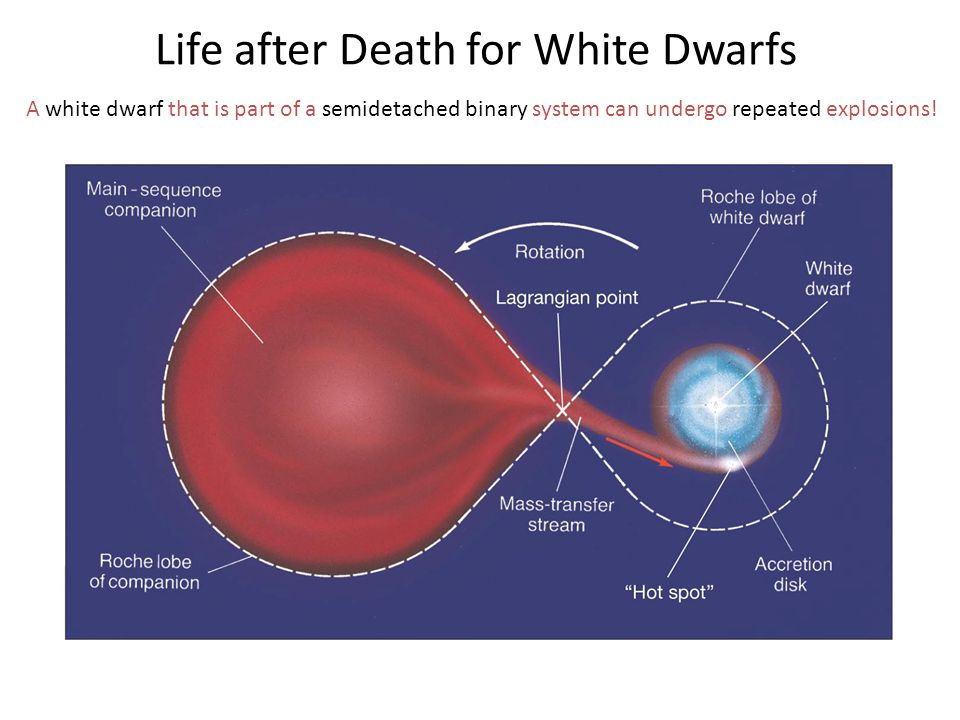
\includegraphics[width=0.8\textwidth]{images/Life+after+Death+for+White+Dwarfs.jpg}
    \caption{Binary system angular momentum transfer through L1.}
    \label{fig:Binary star system L1}
\end{figure}

The matter that flows through the L1 point carries with it angular momentum, as in figure \ref{fig:Binary star system L1}. As this matter accretes onto the recipient star, it can form an accretion disk around the star, and the process of accretion can lead to a redistribution of angular momentum within the system. This can have various effects, such as changing the spin rates of the stars and altering the orbital parameters of the binary system. In extreme cases, this angular momentum transfer can lead to phenomena such as type Ia supernovae.


\subsubsection{Application in back holes}

Matter falling into a black hole experiences significant time dilation due to the extreme curvature of spacetime near a black hole. In any reference frame outside of a black hole, all the matter that has fallen into the black hole (throughout its entire history) is still visible on the surface of the event horizon. However, note that in the reference frame of the infalling particles there is nothing special about the event horizon, matter simply passes right through as if nothing has happened - a consequence of the equivalence principle\footnote{This may not be so simple, see discussions on the firewall paradox in the appendix section \ref{sec:Firewall}}. So there will be a shell of matter surrounding the black holes, as the black holes approach one another, there is a point where the two shells of matter will approach the L1 Lagrange point, hence the matter will momentarily be free of any net gravitational field. This is a point where gravitational reconnection could occur. 

See figure \ref{fig:PE diagram of BBH} for a sketch of the potential energy between two binary black holes. Could there be some flow of matter between the L1 point of this binary, similar to the case of binary stars?

\begin{figure}
    \centering
    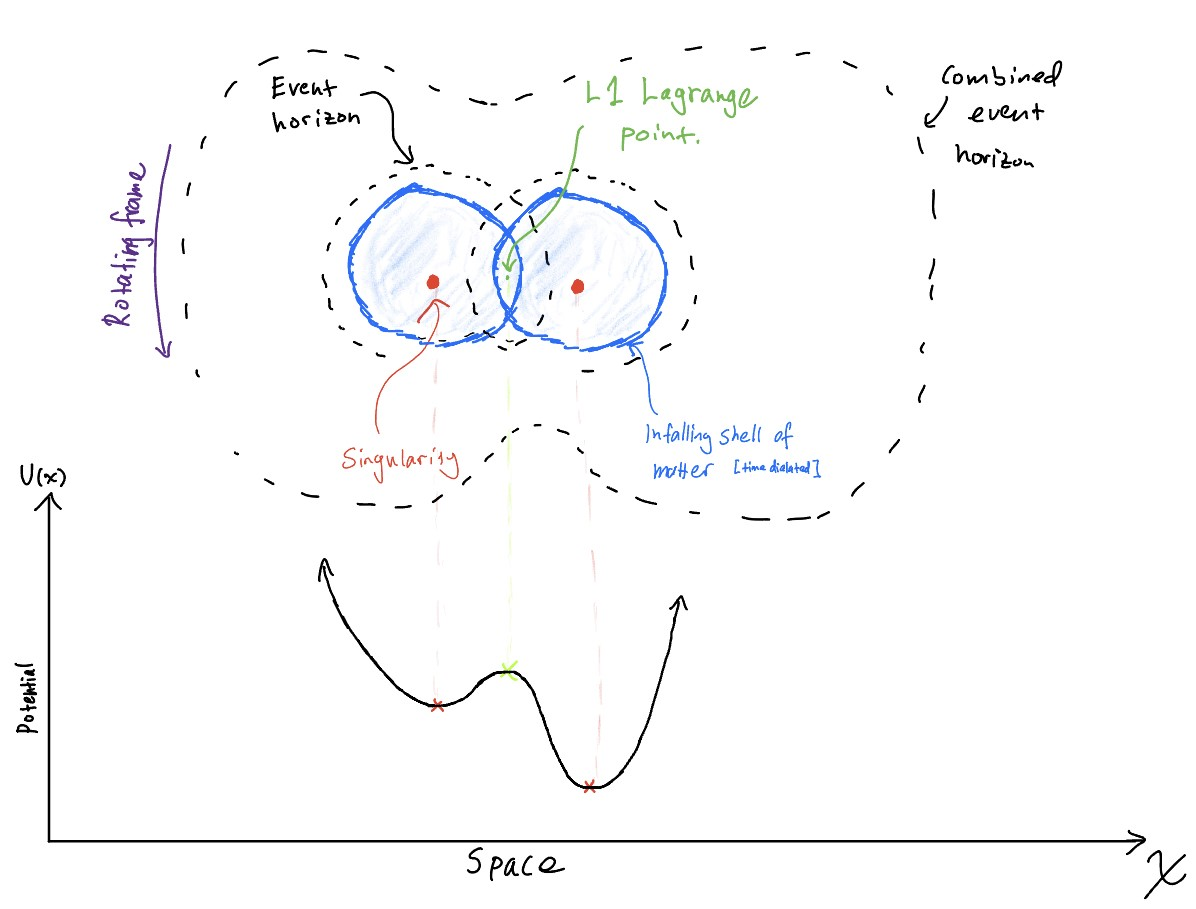
\includegraphics[width=0.75\textwidth]{images/L1_PE.jpeg}
    \caption{Figure shows a potential energy diagram for a binary black hole. Note that there are stable equilibrium points at the singularity, and an unstable equilibrium at the L1 Lagrange point. Can matter channel through this point?}
    \label{fig:PE diagram of BBH}
\end{figure}

\subsubsection{Showing the Lagrange points in Python}

We provide some evidence that the simulator works, at least in the Newtonian case, by simulating some Lagrange points. See figure \ref{fig:Lagrange points in Python}. Note that I can plot the figures in either a inertial frame, showing the rotation of the masses about the origin, or in the rotating frame where the primary and secondary masses are stationary. Most of the figures from here on will be plots in the rotating frame, i.e. the frame where the large masses are stationary.

\begin{figure}
    \centering
     \begin{subfigure}[b]{0.3\textwidth}
         \centering
         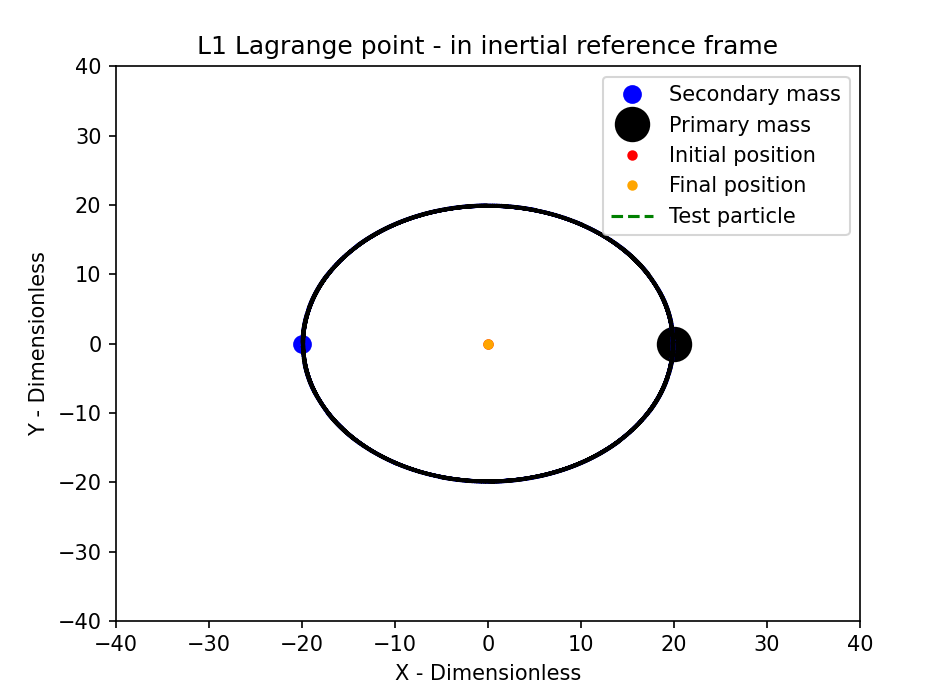
\includegraphics[width=\textwidth]{images/L1 in inertial frame.png}
         \caption{L1 in inertial frame.}
         \label{fig:L1 in inertial frame}
     \end{subfigure}
     \begin{subfigure}[b]{0.3\textwidth}
         \centering
         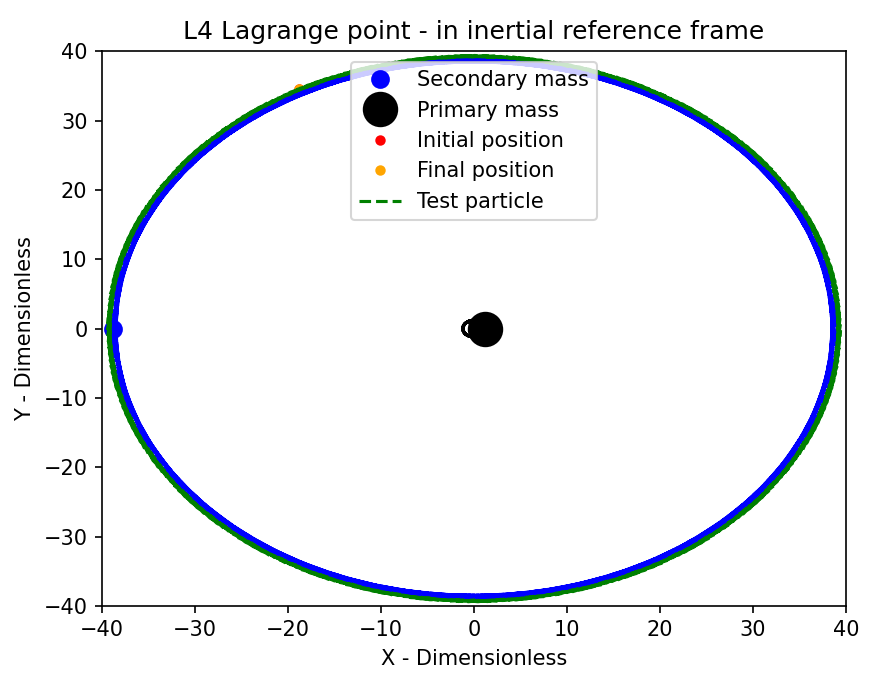
\includegraphics[width=\textwidth]{images/L4 Lagrange point in inertial frame.png}
         \caption{L4 in inertial frame.}
         \label{fig:L4 in inertial frame}
     \end{subfigure}
     \begin{subfigure}[b]{0.3\textwidth}
         \centering
         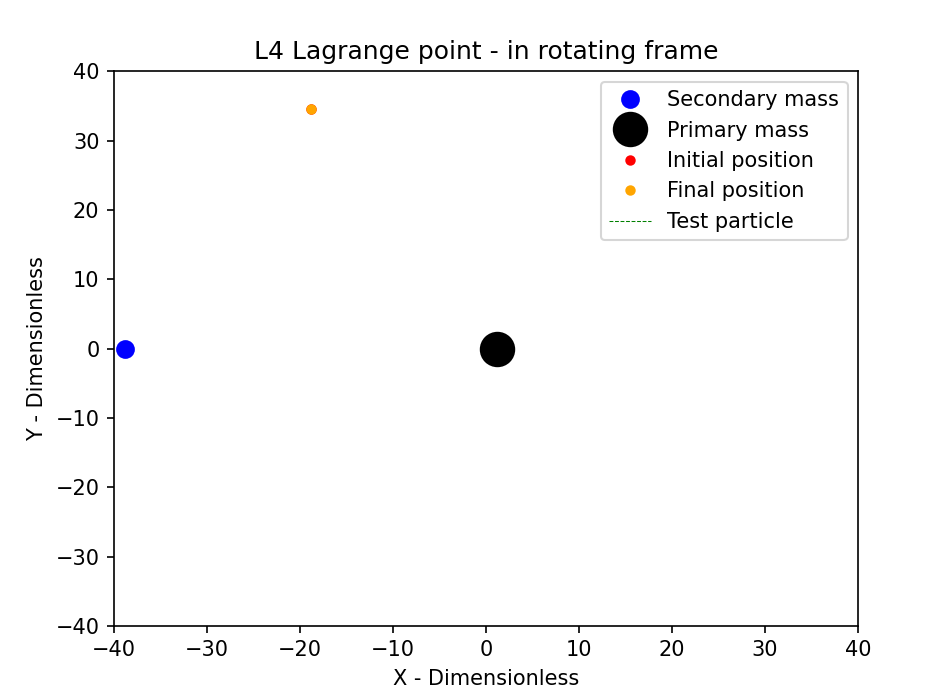
\includegraphics[width=\textwidth]{images/L4 Lagrange point in rotating frame.png}
         \caption{L4 in rotating frame.}
         \label{fig:L4 in rotating frame}
     \end{subfigure}
    \caption{Showing L1 and L4 Lagrange points using my Python program. TODO: Fix images sizes, give better captions. Also made an animation, don't think I can display that in LaTeX.}
    \label{fig:Lagrange points in Python}
\end{figure}


%%%%%%%%%%%%%%%%%%%%%%%%%%%%%%%%%%%%%%%%
%%%%%%%%%% ADD IN GW LOSSES %%%%%%%%%%%%
%%%%%%%%%%%%%%%%%%%%%%%%%%%%%%%%%%%%%%%%

\subsection{Add losses from gravitational waves}
When I add in energy losses from gravitational wave emission, I notice that the location of the  L4 Lagrange point moves closer towards the centre, as shown in figure \ref{fig:L4 with GW losses}. This is explored more in \cite{2010ApJ...724...39S}.

\begin{figure}
    \centering
    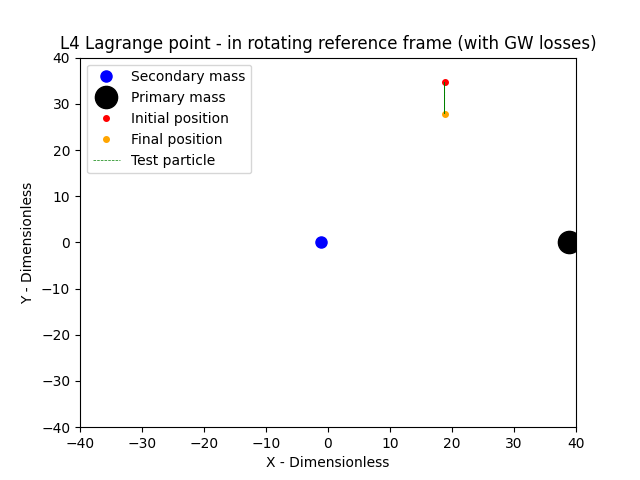
\includegraphics[width=0.5\textwidth]{images/L4 Lagrange point with GW losses.png}
    \caption{Effect of gravitational wave losses on L4 Lagrange point. As you can see, the inspiralling of masses leads to the L4 Lagrange point moving closer to the center (TODO: Be more quantitative with this)}
    \label{fig:L4 with GW losses}
\end{figure}

\subsection{Adding frame dragging}



\begin{figure}
    \centering
    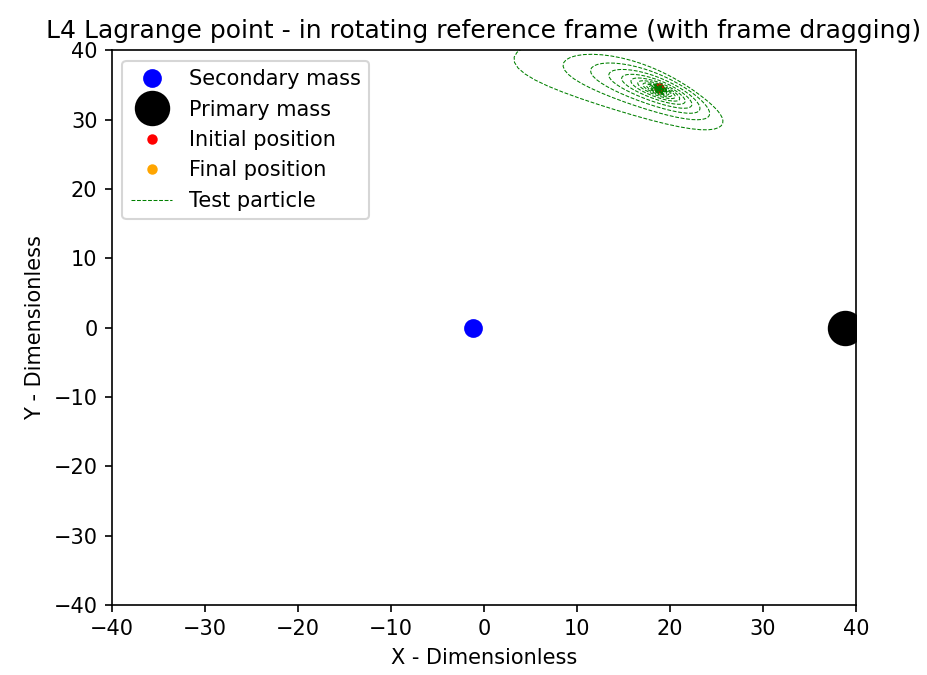
\includegraphics[width=0.75\textwidth]{images/L4 Lagrange point with frame dragging.png}
    \caption{Effect of adding frame dragging on L4 Lagrange point. Spiral behavior reminiscent of charge in magnetic field (as we would expect).}
    \label{fig:L4 with frame draggingl}
\end{figure}

We now add forces on the test particle due to frame dragging, resulting in new behavior for a particle near L4, as shown in figure \ref{fig:L4 with frame draggingl}. The orientation of spins has an appreciable effect on the qualitative behavior of a particle slightly perturbed from the L1 Lagrange point. It appears (TODO: Investigate this thoroughly) that no spin leads to the test particle orbiting the primary mass, aligning the  spins results in particle ejection, and anti-aligning spins causes the particle to fall into the primary mass. The hope of the project would be to show that this behavior is mimicked with actual black holes.

\begin{figure}
    \centering
    \begin{subfigure}[b]{0.3\textwidth}
         \centering
         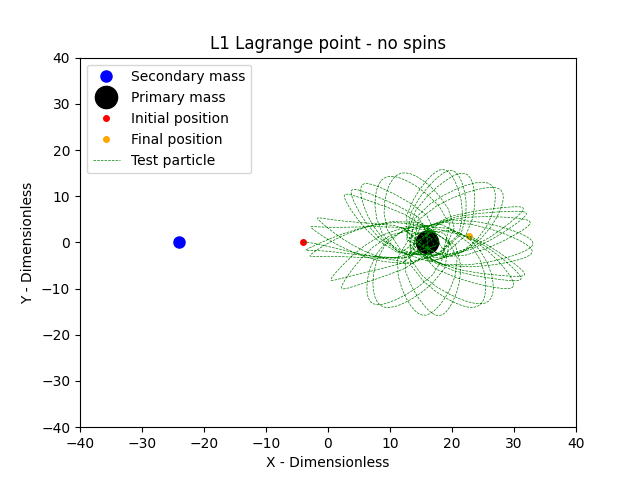
\includegraphics[width=\textwidth]{images/L1 no spin.png}
         \caption{L1 No spin.}
         \label{fig:L1 no spin}
     \end{subfigure}
    \begin{subfigure}[b]{0.3\textwidth}
         \centering
         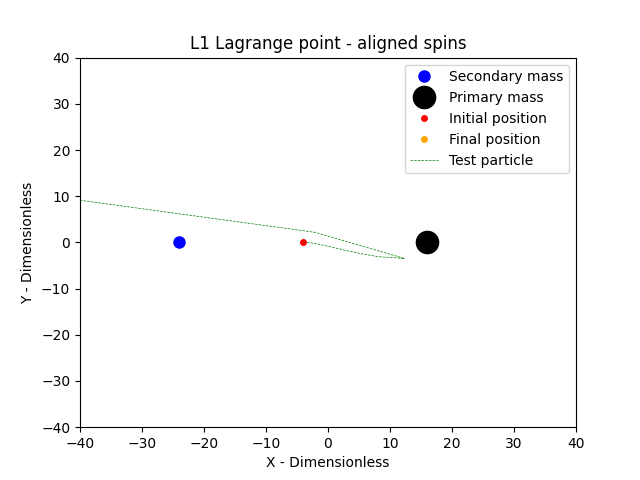
\includegraphics[width=\textwidth]{images/L1 aligned spins.png}
         \caption{L1 aligned spins.}
         \label{fig:L1 aligned spins}
     \end{subfigure}
    \begin{subfigure}[b]{0.3\textwidth}
         \centering
         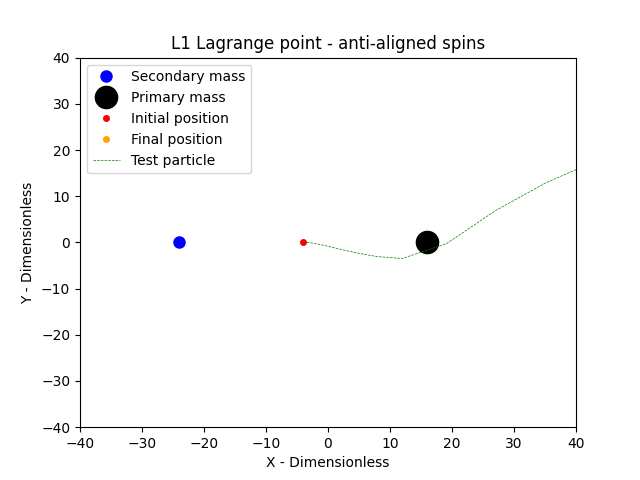
\includegraphics[width=\textwidth]{images/L1 anti-aligned spins.png}
         \caption{L1 anti-aligned spins.}
         \label{fig:L1 anti-aligned spins}
     \end{subfigure}
    \caption{Effect of spin orientation on particle trajectory}
    \label{fig:Spin orientation effect}
\end{figure}

%%%%%%%%%%%%%%%%%%%%%%%%%%%%%%%%%%%%%%%%%%
%%%%%%%%%%   USING PN GRAVITY   %%%%%%%%%%
%%%%%%%%%%%%%%%%%%%%%%%%%%%%%%%%%%%%%%%%%%

\section{Higher order approximations}

To go beyond the basic model, we will use higher order approximations of general relativity. We now use 



%%%%%%%%%%%%%%%%%%%%%%%%%%%%%%%%%%%%%%%%%%
%%%%%%%%%% ANALYTICAL MODELLING %%%%%%%%%%
%%%%%%%%%%%%%%%%%%%%%%%%%%%%%%%%%%%%%%%%%%

\section{Analytical modelling}\label{sec:Analytic}

\subsection{Near fixed point}

We now analyse the stability of the Lagrange points when frame dragging is added. We begin by rewriting the two second order ODEs in equations (\ref{eq:x dot dot}) and (\ref{eq:y dot dot}) as four first order ODES. Defining $v_x=\dot{x}$, and $v_y=\dot{y}$, we get the new system 

\begin{align}
    v_x &= \dot{x}   \notag \\
    v_y &= \dot{y}   \notag \\
    \dot{\omega} &= \frac{96}{5} \mu_1 \mu_2 \omega^{11/3} \notag \\
    \ddot{v}_x &= 2 \omega v_y + \omega^2 x + \dot{\omega} y - \left[ \mu_1 \frac{x+a \mu_2}{r_1^3} + \mu_2 \frac{x-a \mu_1}{r_2^3} \right] + \frac{2 L_2}{r_2^3} v_y \notag \\
    \dot{v}_y &= -2 \omega v_x + \omega^2 y - \dot{\omega} x - \left[ \mu_1 \frac{y}{r_1^3} + \mu_2 \frac{y}{r_2^3} \right] + \frac{2 L_1}{r_1^3} v_x \notag\\
    \boldsymbol{F}(x,y,w,v_x,v_y) &= (v_x, v_y, \dot{\omega}, \dot{v}_x, \dot{v}_y)^{\mathrm{T}} \label{eq: First order sys}
\end{align}

When then obtain the Jacobian matrix $J \equiv D\boldsymbol{F}(x,y,w,v_x,v_y)$ of the system given in equation (\ref{eq: First order sys}), giving the dynamics of the system in the neighbourhood of a point.
    

\[
J = \begin{bmatrix}
    \frac{\partial v_x}{\partial x} & \frac{\partial v_x}{\partial y} & \frac{\partial v_x}{\partial \omega} & \frac{\partial v_x}{\partial v_x} & \frac{\partial v_x}{\partial v_y} \\
    \frac{\partial v_y}{\partial x} & \frac{\partial v_y}{\partial y} & \frac{\partial v_y}{\partial \omega} & \frac{\partial v_y}{\partial v_x} & \frac{\partial v_y}{\partial v_y} \\
    \frac{\partial \dot{\omega}}{\partial x} & \frac{\partial \dot{\omega}}{\partial y} & \frac{\partial \dot{\omega}}{\partial \omega} & \frac{\partial \dot{\omega}}{\partial v_x} & \frac{\partial \dot{\omega}}{\partial v_y} \\
    \frac{\partial \dot{v}_x}{\partial x} & \frac{\partial \dot{v}_x}{\partial y} & \frac{\partial \dot{v}_x}{\partial \omega} & \frac{\partial \dot{v}_x}{\partial v_x} & \frac{\partial \dot{v}_x}{\partial v_y} \\
    \frac{\partial \dot{v}_y}{\partial x} & \frac{\partial \dot{v}_y}{\partial y} & \frac{\partial \dot{v}_y}{\partial \omega} & \frac{\partial \dot{v}_y}{\partial v_x} & \frac{\partial \dot{v}_y}{\partial v_y} \\
\end{bmatrix}
\]

Taking the necessary partial derivatives, we get the Jacobian matrix

\[
J = \begin{bmatrix}
    0 & 0 & 0 & 1 & 0 \\
    0 & 0 & 0 & 0 & 1 \\
    0 & 0 & \frac{352}{5} \mu_1 \mu_2 \omega^{8/3} & 0 & 0 \\
    \omega^2-\frac{\mu_1}{r1^3}-\frac{\mu_2}{r_2^3} & \dot{\omega} & 2 v_y + 2 \omega x & 0 & 2 \omega + \frac{2 L_2}{r_2^3} \\
    -\dot{\omega} & \omega^2 - \frac{\mu_1}{r_1^3}-\frac{\mu_2}{r_2^3} & -2 v_x + 2 \omega y & -2 \omega + \frac{2 L_1}{r_1^3} & 0
\end{bmatrix}
\]

By the \textit{Hartman-Grobman} theorem from dynamical systems, the dynamics near a fixed point $\boldsymbol{x}$ can be identified with the linearized equations $\boldsymbol{F}(\boldsymbol{x}^*+d\boldsymbol{x}) = \boldsymbol{F}(x^*)+D\boldsymbol{F}(\boldsymbol{x}^*) \cdot d\boldsymbol{x}$. To start, consider a system where the masses are equal, $\mu_1=\mu_2=1/2 \implies r_1=r_2=1/2 a$ , we have a fixed point at L1, so by definition $(v_x, v_y, \dot{\omega}, \dot{v_x}, \dot{v_y})=(0,0,0,0,0)$. Thus the Jacobian at this fixed point is given by

\[
J = \begin{bmatrix}
    0 & 0 & 0 & 1 & 0 \\
    0 & 0 & 0 & 0 & 1 \\
    0 & 0 & \frac{352}{5} \mu_1 \mu_2 a^{-4} & 0 & 0 \\
    -7 a^{-3} & 0 & 2 \omega x & 0 & 2 \omega + 16 L_2 a^{-3} \\
    0 &  -7a^{-3} & 2 \omega y & -2 \omega + 16 L_1 a^{-3} & 0
\end{bmatrix}
\]

Where we have written $\omega$ in terms of $a$, according to equation (\ref{eq:kepler's law}). We can now determine the eigenvalues and eigenvectors in order to determine the 
stability of this fixed point under perturbation ...

TODO: Finish off this section.

\subsection{Near primary mass}

To analyse the system near one of the larger masses, we can use perturbation theory ...

TODO: This section.

\subsection{Far from masses}

Then far away from all masses (to determine particle scape) we may be able to use asymptotics ... (not sure about this) ...

TODO: This section.

%%%%%%%%%%%%%%%%%%%%%%%%%%%%%%%%
%%%%%%%%%% NEXT STEPS %%%%%%%%%%
%%%%%%%%%%%%%%%%%%%%%%%%%%%%%%%%

\section{Limitations and next steps}\label{sec:Limitations and next steps}

There are obvious limitations to this study, many of which I have already mentioned. The next step would be to carry out these approximations to either higher post-Newtonan/Minkowski order, or try other analytical techniques like effective one body modelling, or extreme mass ratio inspirals, or other general relativity perturbation methods. I am currently learning about these techniques. The next step after that would be a full numerical relativity simulation, which I am also beginning to learn. One of the resources I am using to learn these topics are the online lectures from the \href{https://www.ictp-saifr.org/the-sound-of-space-time-the-dawn-of-gravitational-wave-science/}{ICTP-SAIFR conference on gravitational waves science}.



\section{Appendix}\label{sec:Appendix}

\subsection{Python code for basic model}\label{sec:Python code}

Below is the code used to simulate the equations of motion of the simple model considered.


\begin{mintedbox}{python}
import numpy as np
import matplotlib.pyplot as plt
from scipy.integrate import solve_ivp
from matplotlib.animation import FuncAnimation

# TODO: Add in code for making plots, or just link github

def EOM(t, f, mu1, mu2, a, GW_losses, L1, L2):
    """Equations of motion inside rotating reference frame. Can optionally include damping due to gravitational waves losses 
        and frame dragging effects."""

    x, y, z, w, vx, vy, vz = f

    # These would be constant at a lagrange point
    r1 = np.sqrt((x+a*mu2)**2 + y**2 + z**2)
    r2 = np.sqrt((x-a*mu1)**2 + y**2 + z**2)
    r = np.sqrt(x**2 + y**2 + z**2)

    # Equations of motion
    vw = (96/5)*mu1*mu2*w**(11/3) if GW_losses else 0.0
    ax = 2*w*vy + w**2*x + vw*y - (mu1*(x+a*mu2))/(r1**3) - (mu2*(x-a*mu1))/(r2**3)
    ay = -2*w*vx + w**2*y - vw*x - (mu1*y)/(r1**3) - (mu2*y)/(r2**3)
    az = -mu1*z/(r1**3) - (mu2*z)/(r2**3)

    v = np.array([vx, vy, vz])
    Bg = 0.5 * (-L1 / r1**3 + L2 / r2**3) * np.array([0, 0, 1])
    ag = 4*np.cross(v, Bg)
    ag_x, ag_y, ag_z = ag[0], ag[1], ag[2]
    
    # # Frame dragging
    # ag_x = (2*L2 / r2**3) * vy              # Acceleration due to frame dragging, in x direction
    # ag_y = (2*L1 / r1**3) * vx              # Acceleration due to frame dragging, in y direction
    # ag_z = 0
    
    ax += ag_x
    ay += ag_y
    az += ag_z

    dfdt = [vx, vy, vz, vw, ax, ay, az]

    return dfdt


def simulate(mu, a, f0, GW_losses, num_periods=10, L1=0, L2=0):
    """
    mu = fraction of total mass in larger mass object, e.g. mu = 0.9 means mu1 = 0.1 and mu2 = 0.1
    a = semi-major axis
    f0 = [x0, y0, z0, vx0, vy0, vz0] is initial position and velcocity
    num_periods = number of periods of binary orbits to simulate for
    """

    mu2 = mu
    mu1 = 1 - mu2
    
    # Angular velocity, given by Kepler's third law (with G=c=1)
    w = a**-1.5
    f0 = f0[:3] + [w] + f0[3:]


    # Define time span
    t0 = 0
    orbital_period = 2*np.pi*a**1.5
    T = num_periods * orbital_period

    # Solve ODE

    sol = solve_ivp(EOM, [t0, T], f0, args=(mu1, mu2, a, GW_losses, L1, L2), method='RK45', dense_output=True, rtol=1e-10, atol=1e-10)

    # Extract positions and plot orbit
    x = sol.y[0]
    y = sol.y[1]
    z = sol.y[2]
    w = sol.y[3]
    vx = sol.y[4]
    vy = sol.y[5]
    vz = sol.y[6]

    return x, y, z, w, vx, vy, vz


def plot(mu, a, f0, GW_losses, num_periods=10, reference_frame="rotating", title="Orbit", L1=0, L2=0):
    
    x, y, z, w, vx, vy, vz = simulate(mu, a, f0, GW_losses, num_periods=num_periods, L1=L1, L2=L2)
        
    fig, ax = plt.subplots()
    
    ax.set_title(title)
    ax.set_xlabel("X - Dimensionless")
    ax.set_ylabel("Y - Dimensionless")
    ax.set_xlim(-a, a)
    ax.set_ylim(-a, a)
    
    # Plot two primary masses
    ax.plot(-a*mu2, 0, 'o', color='blue', markersize=8, label="Secondary mass")
    ax.plot(a*mu1, 0, 'o', color='black', markersize=16, label="Primary mass")

    # Plot initial and final position of test particle
    ax.plot(x[0], y[0], 'o', color='red', markersize=4, label = "Initial position")
    ax.plot(x[-1], y[-1], 'o', color='orange', markersize=4, label = "Final position")
    
    
    if reference_frame == "inertial":
        t0 = 0
        orbital_period = 2*np.pi*a**1.5
        T = num_periods * orbital_period
        num_timesteps = len(x)
        t = np.linspace(t0, T, num_timesteps)

        # Convert to inertial frame
        X = +x*np.cos(w*t) + y*np.sin(w*t)
        Y = -x*np.sin(w*t) + y*np.cos(w*t)
        
        # Plot particle motion, in non rotating (inertial) reference frame
        ax.plot(X, Y, label='Test particle', color='green', ls='--')
        
        # Plot motion of binary objects
        ax.plot(-a*mu2*np.cos(w*t), -a*mu2*np.sin(w*t), ls='--', color='blue')
        ax.plot(a*mu1*np.cos(w*t), a*mu1*np.sin(w*t), ls='--', color='black')

    elif reference_frame == "rotating":
        ax.plot(x, y, label='Test particle', color='green', ls='--', linewidth=0.5)
    else:
        raise ValueError('Choose reference_frame="rotating" or reference_frame="inertial"')
        
    
    ax.legend()
    plt.title(title)
    
    return fig, ax

def animate_trajectories(mu, a, f0, GW_losses, num_periods=10, title="Orbit", L1=0, L2=0, reference_frame="rotating"):
    
    x, y, z, w, vx, vy, vz = simulate(mu, a, f0, GW_losses, num_periods=num_periods, L1=L1, L2=L2)
    
    t0 = 0
    orbital_period = 2*np.pi*a**1.5
    T = num_periods * orbital_period
    num_timesteps = len(x)
    t = np.linspace(t0, T, num_timesteps)
    
    # Convert to inertial frame
    X = x*np.cos(w*(-t)) + y*np.sin(w*(-t))
    Y = -x*np.sin(w*(-t)) + y*np.cos(w*(-t))

    # Create the figure and axes
    fig, ax = plt.subplots()
    ax.set_title(title)
    ax.set_xlabel("X - Dimensionless")
    ax.set_ylabel("Y - Dimensionless")
    ax.set_xlim(-a, a)
    ax.set_ylim(-a, a)

    # Plot two primary masses (initial position)
    mass1, = ax.plot(-a*mu2*np.cos(w*t[0]), -a*mu2*np.sin(w*t[0]), 'o', color='blue', markersize=10)
    mass2, = ax.plot(a*mu1*np.cos(w*t[0]), a*mu1*np.sin(w*t[0]), 'o', color='black', markersize=30)

    # Plot initial position of test particle
    particle, = ax.plot(X[0], Y[0], 'o', color='red', markersize=5)

    # Function to update the positions
    def update(i):
        mass1.set_data(-a*mu2*np.cos(w*t[i]), -a*mu2*np.sin(w*t[i]))
        mass2.set_data(a*mu1*np.cos(w*t[i]), a*mu1*np.sin(w*t[i]))
        particle.set_data(X[i], Y[i])

    # Create the animation
    ani = FuncAnimation(fig, update, frames=range(0, num_timesteps), interval=300)

    return ani


# Stability of L4

mu = 0.97
mu2, mu1 = mu, 1-mu
a = 40
x0 = (-a*mu2+a*mu1)/2
y0 = (a*mu2+a*mu1)*np.sqrt(3)/2
z0 = 0.0
vx0 = 0.000
vy0 = 0.0
vz0 = 0.0
f0 = [x0, y0, z0, vx0, vy0, vz0]
GW_losses = True
L1 = 1
L2 = 1

# Add in code for more figures.

plot(mu, a, f0, GW_losses, num_periods=10, L1=L1, L2=L2, reference_frame="rotating", title="In rotating reference frame")

ani = animate_trajectories(mu, a, f0, GW_losses, num_periods=10, L1=L1, L2=L2, reference_frame="rotating", title="In rotating reference frame")

plt.show()
\end{mintedbox}

\subsection{ER = EPR}
Don't bother reading this section, I need to rewrite this.


\subsubsection{The paradox}

Emission of Hawking radiation from a black holes results in entangled pairs of radiation. Think of pair production, where conservation of spin results in the spins being of opposite orientation, hence knowing the spin of one photon tells you the spin of the other - i.e. the photons are entangled. The principle of monogamy in quantum mechanics states that particles can only be entangled with one other particle. However, what about when the radiation in the first black hole is emitted during the evaporation of the black hole? It cannot be both entangled with the Hawking radiation emitted in the past and the black hole behind the event horizon (which it must, from quantum information theory, which is required to save unitarity in quantum mechanics). Thus a paradox. 

\subsubsection{AMPS and firewalls}\label{sec:Firewall}

A 2012 paper by Ahmed Almheiri, Donald Marolf, Joseph Polchinski, and James Sully proposed the "firewall" resolution to this paradox. They suggested that somehow entanglement between the in-going and outgoing radiation is broken as a particle crosses the event horizon, this breaking of entanglement releases a large amount of energy, creating a "firewall" around the event horizon. This principle violates Einstein's equivalence principle, which implies that there is nothing special about the event horizon. Einstein's equivalence principle states that all reference frames are locally inertial, hence an observer free falling past the event horizon will experience nothing special. This contradicts the firewall resolution, which says the in-falling observer will be incinerated by the firewall.

\subsubsection{ER=EPR resolution}

In 2013 Susskind (String theory guy) and Maldacena (ADS/CFT guy) proposed a resolution which - unlike all other proposed solutions - did not violate the unitarity of quantum mechanics, Einstein's equivalence principle, or existing quantum field theory. It did however, require the use of wormholes. An Einstein-Rosen bridge is a solution of Einstein's field equations that connects distant regions of spacetime. There is no contradiction with special relativity, a particle cannot enter a Einstein Rosen bridge and escape to the other side of the wormhole (since the wormhole is a black hole), so faster than light travel between points in space is not allowed. This can be seen from the Penrose diagram in figure \ref{fig:womhole penrose diagram}.ER = EPR conjectures that two entangeled particles (a Einstein-Podolsky-Rosen or EPR pair) are connected by an Einstein-Rosen (ER) bridge, i.e. the holographic dual (see the holographic principle and ADS/CFT correspondence) to particle entanglement is a wormhole.

\begin{figure}
    \centering
    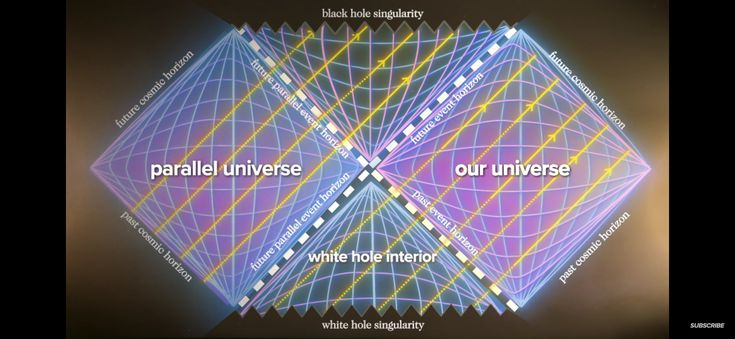
\includegraphics[width=0.5\textwidth]{images/8f24704956231dec3a4e849f60a54687.jpg}
    \caption{Penrose diagram of wormhole. Recall on Penrose diagrams that diagonal lines represent particles moving at the speed of light, so there is no way to connect the left region with the right. Particles from the two separated regions can however meet inside the black hole and exchange information.}
    \label{fig:womhole penrose diagram}
\end{figure}

\subsection{Binary black hole exploration and silly ideas/questions}

\begin{enumerate}
    \item Question about spacetime entanglement/EPR explanation
    \item Is there a Penrose diagram for binary black holes?
    \item Can super-radiance be used to amplify hawking radiation between binary black holes?
    \item When BBHs collide, can particles originally in one horizon end up in the singularity of the other (most likely the singularities will merge before the particle can enter either singularity). This would be similar to L1 accretion in binary stars.
    \item Bruce's question on particle at L1 escaping event horizon.
\end{enumerate}


\printbibliography

\end{document}
